% Chapter 3

\chapter{Transferencia de aprendizaje} % Main chapter title

\label{Chapter3} % For referencing the chapter elsewhere, use \ref{Chapter1} 

En este capítulo se cubren y se fundamentan las técnicas de transferencia de aprendizaje (transfer learning) usadas y las decisiones tomadas para el diseño del proyecto de clasificación de autores con redes neuronales recurrentes.

\section{Transferencia de aprendizaje} % Main chapter title

Un concepto esencial para este trabajo y para toda el área de Deep Learning, es la capacidad de transferir aprendizaje adquirido previamente de un problema poco acotado y aprovechar este aprendizaje en problemas más acotados, al permitir así que las demandas de recursos como datos y tiempo de ejecución tengan más holgura. Se obtienen mejores resultados en menos tiempo al transferir aprendizaje de un modelo que cuando se inicializan los pesos de los parámetros de la red aleatoriamente \parencite{Erhan:2010:WUP}.

\section{Concepto de transferencia}

Las redes neuronales capturan diferente información en sus capas \parencite{yosinski:2014, zeiler2014visualizing} y la forma en que difieren permite transferir conocimiento a través de redes entrenadas para diferentes tareas. En las primeras capas se aprende información bastante abstracta con respecto a la tarea, y conforme se avanza en la profundidad de la red se vuelve más específica la información que se va aprendiendo. Debido a esto se puede utilizar lo aprendido en las primeras capas para otra tarea del mismo dominio.

\begin{figure}
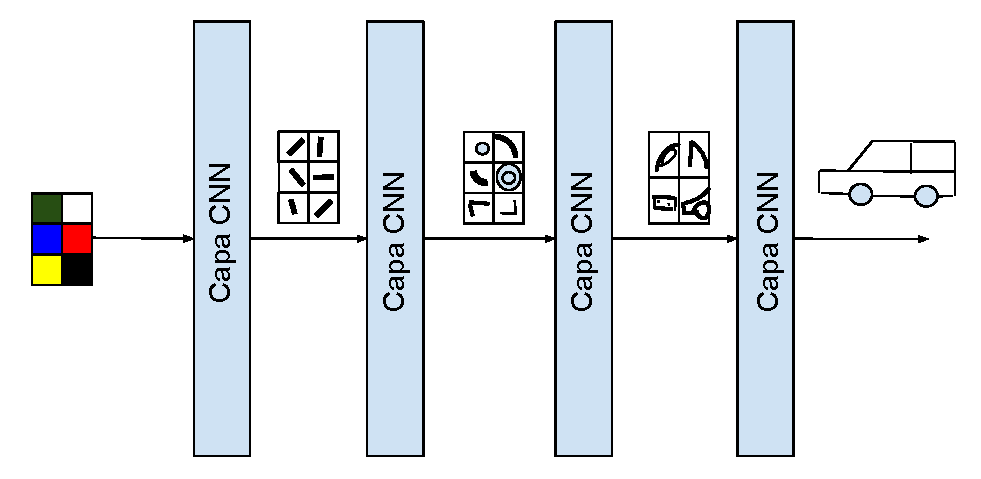
\includegraphics[scale=1]{Figures/learnbylayer.pdf}
\caption{Ejemplo ilustrativo de lo que podría aprender una red profunda de visión artificial para la detección de vehículos.}
\label{fig:learnbylayer}
\end{figure}

\textbf{Ejemplo ilustrativo.} En una red neuronal, cuya tarea es en el área de visión artificial las primeras capas comienzan a entender conceptos de orillas horizontales o verticales; las siguientes capas podrán entender qué son esquinas circunferencias; las siguientes capas podrán entender límites de objetos; etc.

La información en las primeras capas de una red neuronal de visión artificial puede llegar a ser muy útil, sin importar la tarea final o qué tan acotada esté. Por esta razón es posible tomar un modelo pre-entrenado en una tarea general, remover su capa final --- que determina el resultado final de esa tarea en específico --- y continuar con el proceso de entrenamiento con datos de la tarea más acotada y permitir que las nuevas capas no entrenadas aprovechen los conceptos de las capas anteriores para que ellas tengan el poder de predecir al usar esa información y los resultados correctos.



\section{Aplicación en CV}
%Incluir trabajos relacionados
Para tener el contexto acerca de este concepto crucial para este trabajo debemos explorar otras áreas del Deep Learning, en particular el área de visión artificial (computer vision en inglés). Este campo fue el que llevó a la explosión de Deep Learning en el 2012, cuando una red denominada AlexNet dominó la competencia de clasificar el dataset ImageNet \parencite{deng2009imagenet}.

\textbf{ImageNet.} Este proyecto es una colección masiva de imágenes que están debidamente etiquetadas con cuadros encerrando los objetos detectados en una imagen. Debido a la cantidad exagerada de categorías y objetos encontrados en las imágenes y también la cantidad en sí de imágenes, se organiza un concurso de software todos los años para determinar cuál modelo es el mejor en visión artificial. Cuando en el 2012 una red de Deep Learning ganó el concurso se generó motivación en explorar este campo más a fondo.

Esta tarea llegó a ser el estándar para determinar si un modelo podía \emph{ver} a nivel general. ¿Qué significa esto? La tarea de ver es una tarea muy basta y bastante general. Hay muchas características por considerar, lo que aumenta la complejidad de este problema.

% incluir ilustracion de imagenet aca

En CV existen muchas más tareas más acotadas que ver. Para estas sería muy útil utilizar información previamente aprendida con la finalidad de no necesitar muchos datos para la tarea más específica. Por su misma naturaleza, tendrá menos datos de entrenamiento.

\section{Aplicación en NLP}

Hasta el año 2018 no se había aplicado la transferencia de aprendizaje en el área de NLP, pero eso cambió después de trabajos pioneros \parencite{peters:2018, howard2018, devlin2018bert} la técnica muestra promesa. Se podría decir que el momento ImageNet ha llegado a NLP y el progreso ha sido de crecimiento explosivo.

La tarea general en NLP para tener un modelo base ha sido la tarea del modelo de lenguaje \parencite{howard2018}. Un modelo de lenguaje es el que intenta predecir la próxima palabra tomando en cuenta las palabras mandadas como argumento al modelo. En textos de temas específicos esto podrá resultar ser un tanto más fácil debido al vocabulario más limitado y por tener acotado el tema. Idealmente para tener una generalización poderosa y que puede aportar en tareas de muy distintos campos, se debe tener un modelo de lenguaje aprendido de un corpus de datos amplio y la cantidad de textos deberá ser masiva.

Un corpus que cumple con los requisitos mencionados sería la versión de Wikipedia en el lenguaje deseado. La enciclopedia virtual abarca muchos temas y tiene diversidad incomparable de vocabulario. Incluso deberá ser limitado a una cantidad $T$ de tokens. En futuros trabajos se deberá explorar la posibilidad de utilizar distintos corpora.

El modelo de lenguaje es entrenado al usar redes neuronales recurrentes en alguna variante que se considere prudente. Una red LSTM o una \gls{qrnn} \parencite{bradbury2016} son ideales para propósitos de este trabajo y han mostrado los mejores resultados del estado del arte en modelos de lenguaje.

\subsection{ULMFiT}

Esta técnica expuesta originalmente por \textcite{howard2018}, en su curso de Deep Learning, fue publicado para plantear el algoritmo de forma más formal y con estudios de ablación demostrar que cada aspecto de los pasos es esencial para obtener los mejores resultados. La técnica de \gls{ulmfit} se divide en dos fases \parencite{howard2018} las que se explicarán a continuación.

\subsubsection{Afinación de modelo de lenguaje}
\label{lmftune}

Esta fase de la técnica consiste en tomar el modelo de lenguaje general y afinarlo para que esté orientado a la tarea final específica con la que se trabajará. Esto se logra al utilizar los datos de la tarea final para formar un texto sobre el que se terminará de entrenar. Para lograr este afinamiento de la mejor manera, se utilizan diferentes técnicas.

\textbf{Afinamiento discriminatorio.} Esta técnica llamada \textit{fine-tuning}, en el artículo original, consta en usar una tasa de aprendizaje diferente a lo largo de las capas. Es decir, cada capa tiene asignada una tasa de aprendizaje distinta. Se define entonces que los parámetros serán divididos en ${\theta^1, \ldots, \theta^L}$ donde $L$ es el número de capas y $\theta^t$ es el conjunto de parámetros de la capa $l$. La actualización de los parámetros entonces, basado en la ecuación \ref{eq:sgdupdate}:

\begin{equation}
\label{eq:discupdate}
\theta_t^l = \theta_{t-1}^l - \gamma^l \nabla_{\theta} L(\theta)
\end{equation}

\textbf{Tasa de aprendizaje en triangulo inclinado.} Llamado \emph{slanted triangle learning rates} en el artículo original. Durante el recorrido a través de los datos se varía la tasa de aprendizaje tal que su valor aumente durante las primeras $cut$ instancias donde,

$$ cut = \lfloor T \cdot cut\_frac \rfloor$$

$cut\_frac$ es la fracción de datos que queremos sean aprendidos con el crecimiento de la tasa de aprendizaje. Después de que este porcentaje es alcanzado, la tasa de aprendizaje deja de incrementar en valor y empieza a disminuir de forma menos acelerada hasta que se termina de iterar sobre los datos de entrenamiento.

\subsubsection{Afinación de modelo a tarea de clasificación}

Para afinar el modelo de la tarea de clasificación se deberá aplicar el mismo pre-procesamiento en cuanto a tokens de vocabulario. Tener el modelo pre-entrenado y afinado permite obtener resultados bastante precisos, sin necesidad de tener muchos datos de entrenamiento para la tarea específica.

Para el afinamiento de este modelo se aplican los conceptos desarrollados en la sección \ref{lmftune}. Adicionalmente se utiliza una técnica que previene la pérdida de conocimiento.

\textbf{Descongelamiento gradual.} Llamado \emph{gradual unfreezing} en el artículo original. Esta técnica es de las más importantes. El concepto de transferencia de aprendizaje se basa en no perder conocimiento aprendido desde la tarea general original. Al refinar un modelo completamente se toma gran riesgo de \emph{olvidar} vasta información. Esta técnica propone congelar los pesos de todas las capas e ir descongelando una por una y después ajustar y entrenar todas las capas descongeladas. Iterando sobre esto hasta que ya no hay capas por descongelar y se termina de afinar el modelo completo.

\subsection{Modelo de lenguaje bidireccional}

Existe la posibilidad de volver el modelo de lenguaje en un modelo bidireccional \parencite{howard2018}. Esto se puede hacer de forma manual, al revertir el orden de los textos en el corpus y entrenar de la misma forma. Al tener ambos modelos listos se pueden promediar los resultados de las predicciones de cada modelo para obtener la predicción final.

Esto ha sido denominado como modelo bidireccional poco profundo o superficial \parencite{devlin2018bert}. Esto no es debido porque no es un modelo de Deep Learning, sino que la representación en ambas direcciones no está presente en el modelo, sino se logra con el resultado de dos modelos unidireccionales independientes.
